\begin{center}
\vspace*{0.1in}
\begin{Large}
\textbf{PRACTICA DE LABORATORIO N° 02:} \\
\textbf{(Modelando Datos en Power BI)} \\
\end{Large}
\end{center}
\begin{document}
\section{OBJETIVO:}
\item{
Desarrollar el Informe de Labratorio 02 de Modelando Datos en Power BI}
\section{REQUERIMIENTOS}
\begin{itemize}

- Conocimientos básicos de administración de base de datos Microsoft   SQL Server.
\\- Conocimientos básicos de SQL.
\\- Microsoft SQL Server 2016 o superior
\\- Base de datos AdventureWorks2016 o superior
\\- Power BI Desktop.
\\- Tener una cuenta Microsoft registrada en el Portal de Power Bi.
\end{itemize}
\section{CONSIDERACIONES INICIALES}
\item{Generar una carpeta o directorio Power BI en un lugar accesible para guardar los resultados de la práctica.}\\

\section{DESARROLLO}
\newpage
\subsection{IMAGEN Nº01:}
\begin{itemize}
Ingresar a Power BI Desktop, en el cuadro de dialogo Obtener Datos (Get Data), asegurarse que Excel esta seleccionado y hacer click en Conectar (Connect), buscar el archivo Adventure Works Sales Data.xlsx y hacer click en Cargar (Load).

\end{itemize} 

\begin{figure}[httb]
\begin{center}
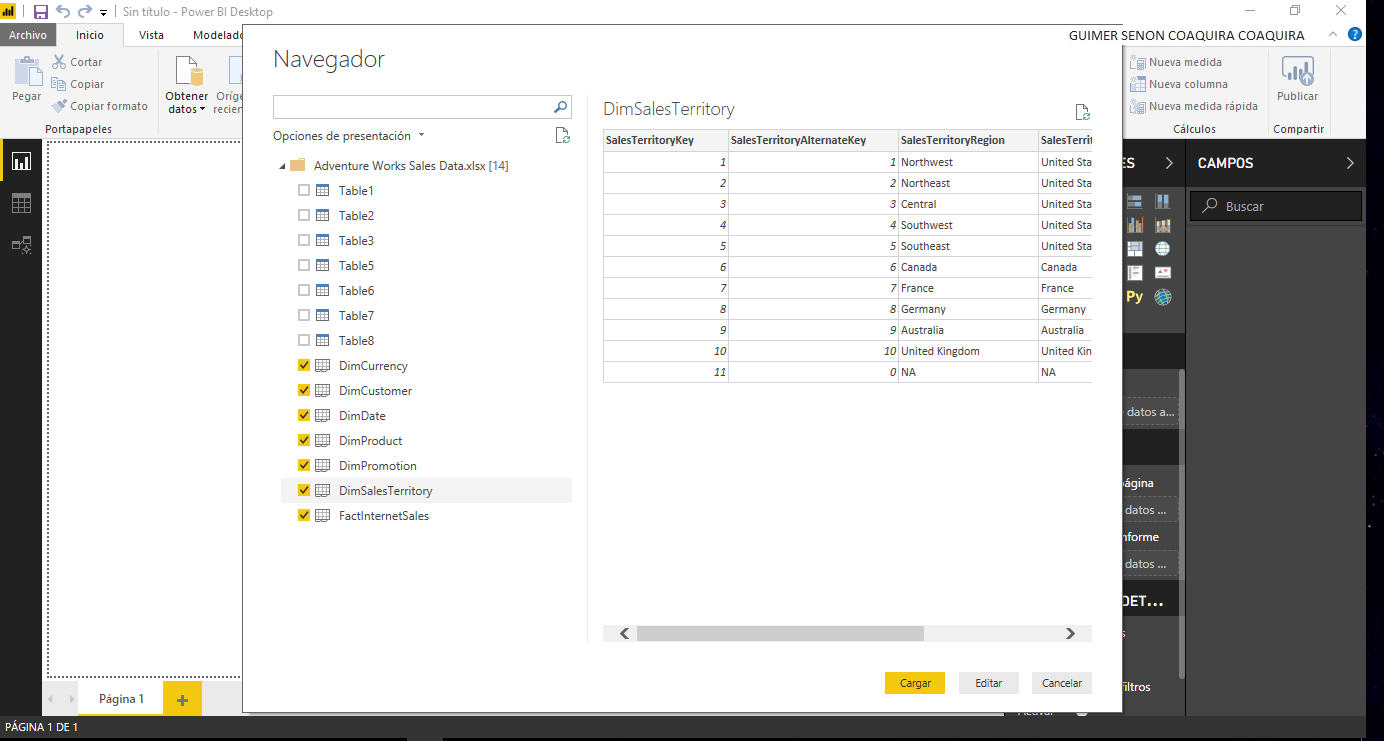
\includegraphics[width=13cm]{./Imagenes/Captura01}
\end{center}
\end{figure}

\subsection{IMAGEN Nº02:}
\begin{itemize}
En el cuadro de Administrar relaciones (Manage Relationships) realizar las configuraciones indicadas 
\end{itemize} 

\begin{figure}[httb]
\begin{center}
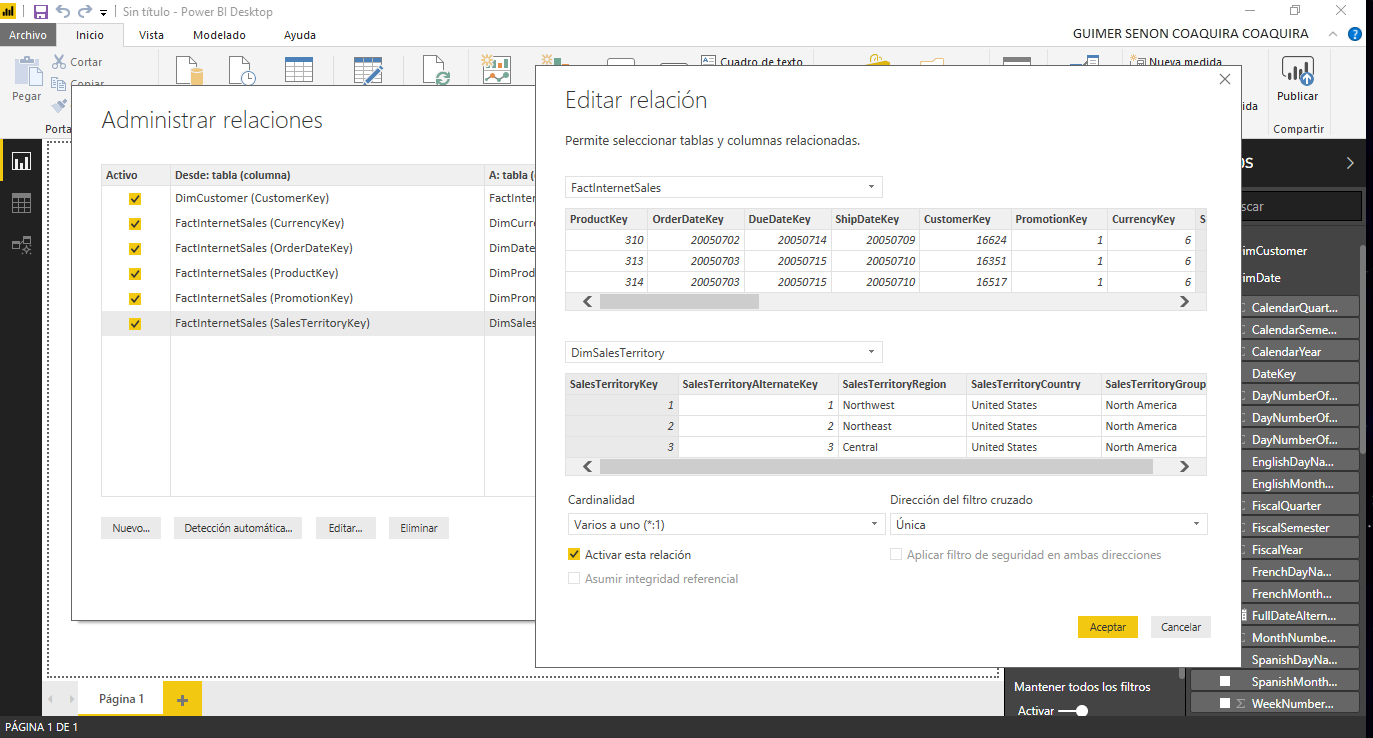
\includegraphics[width=13cm]{./Imagenes/Captura02}
\end{center}
\end{figure}
\newpage
\subsection{IMAGEN Nº03:}
\begin{itemize}
Abrir el archivo Adventure Works Product Categories.xlsx
\end{itemize} 

\begin{figure}[httb]
\begin{center}
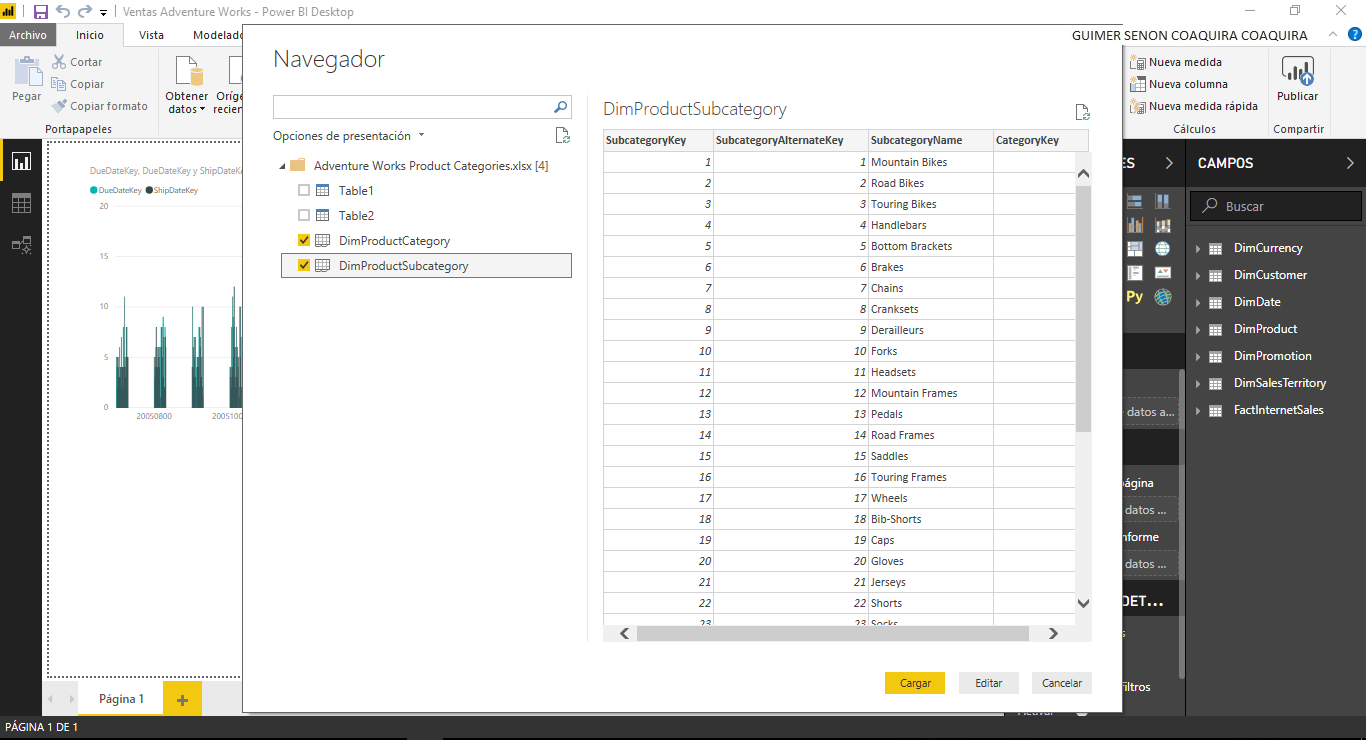
\includegraphics[width=13cm]{./Imagenes/Captura04}
\end{center}
\end{figure}



\subsection{IMAGEN Nº04:}
\begin{itemize}
En el panel Campos, haga clic en DimCustomer,en la cinta Modelado, en el grupo Cálculos, haga clic en Nueva columna.En la barra de fórmulas, resalte Columna = y escriba:
IncomeStatus = IF (DimCustomer[YearlyIncome] < 25000, "Lower Income",
IF (AND(DimCustomer[YearlyIncome] >= 25000, DimCustomer[YearlyIncome] < 60000),
"Middle Income",
IF (AND(DimCustomer[YearlyIncome] >= 60000, DimCustomer[YearlyIncome] < 100000),
"Higher Income",
IF (DimCustomer[YearlyIncome] >= 100000, "Very High Income", "Other")))) y finalmente presione Enter.
\end{itemize}

\begin{figure}[httb]
\begin{center}
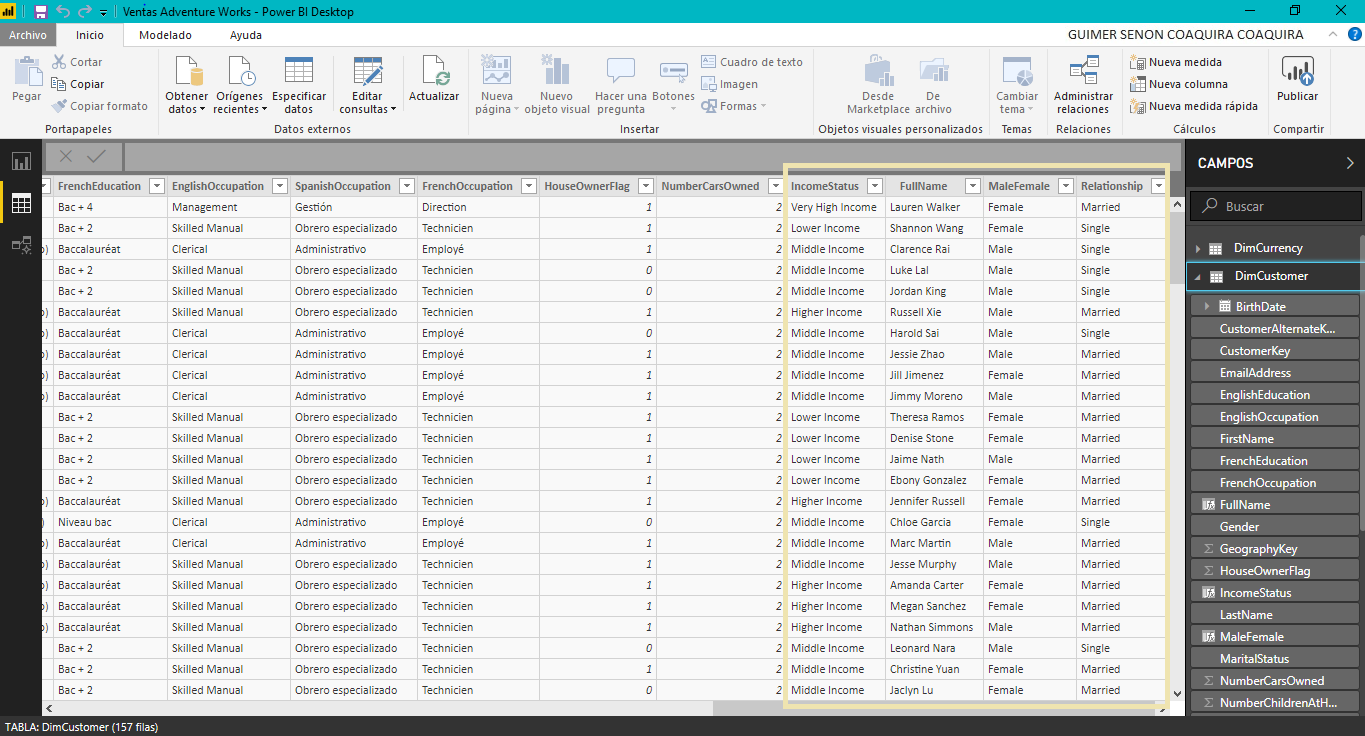
\includegraphics[width=13cm]{./Imagenes/Captura06}
\end{center}
\end{figure}

\newpage
\subsection{IMAGEN Nº05:}
\begin{itemize}
En el panel Campos, haga clic en FactInternetSales.En la cinta Modelado, en el grupo Cálculos, haga clic en Nueva columna y realizar la siguiente operacion:
Profit = CURRENCY(FactInternetSales[UnitPrice] -
FactInternetSales[ProductStandardCost])
\end{itemize}

\begin{figure}[httb]
\begin{center}
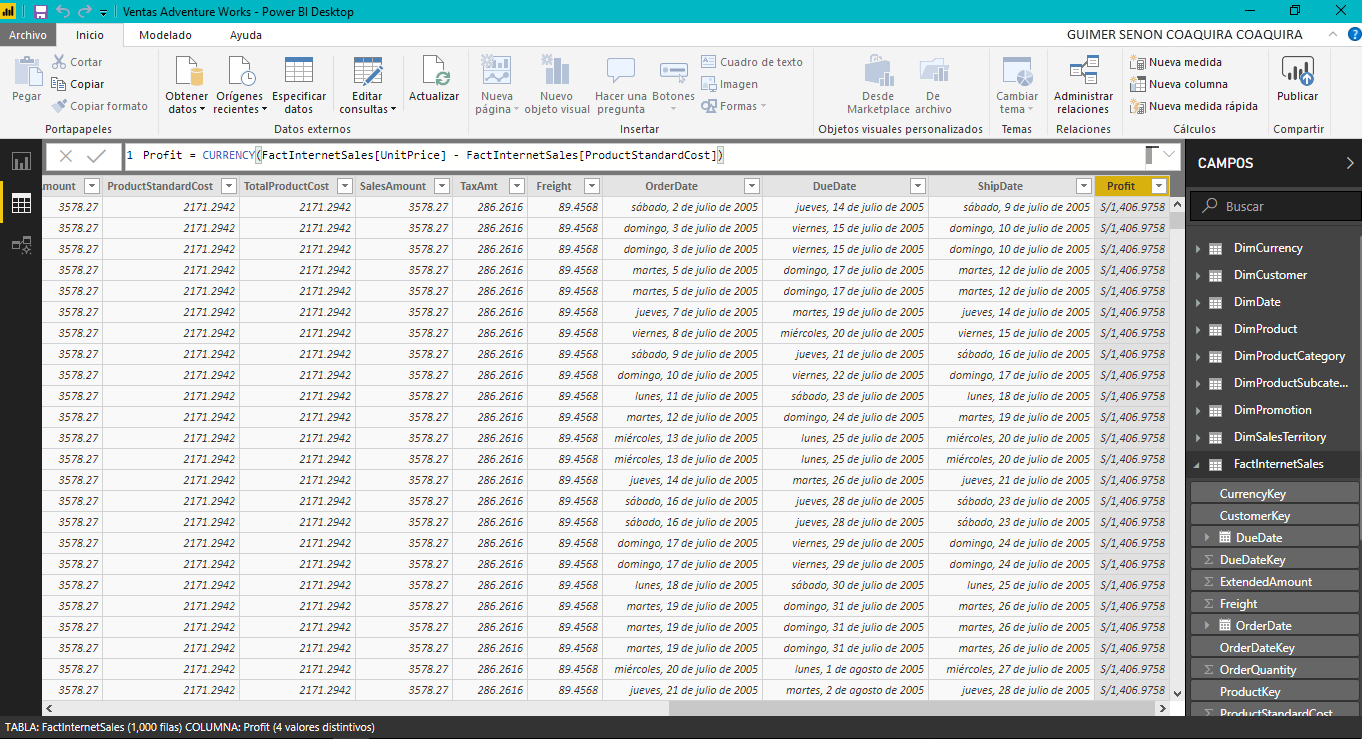
\includegraphics[width=13cm]{./Imagenes/Captura08}
\end{center}
\end{figure}